%!TEX root = ../munich21.tex

%\section{Even finer invariants}
\note{Let's discuss some even finer invariants of the cohomology of spaces}

\begin{frame}{Secondary operations}
	\note{Steenrod squares are defined by the cup-$i$ products which arise from lifting to the cochain level the commutativity relation of the cup product in cohomology. Recall, that the coboundary of cup-1 is the difference between cup-0 and its transpose.

	We are motivated then to look for other cohomological relations to lift.

	We look at Steenrod squares themselves, sometimes referred to as primary cohomology operations. They satisfy relations and the invariants that appear by lifting and solving these relations are known as secondary operations. \press

	There are two main relations that Steenrod squares satisfy: The Cartan and Adem relations. The first tells us how the squares interact with the cup product and the second tells us about their behaviour under interation. \press

	Can we lift these relations the cochain level?

	Yes, the cup-$i$ products can be used to define both, the squares and the cup product in cohomology, so we use them to express these relations in the form: cup-$i$ version of the left hand side minus cup-$i$ version of the right hand side equal to a coboundary \press

	So we wonder if we can solve these equation, effectively constructing such coboundaries, and unlocking secondary cohomology operations
}

	The $Sq^k$ are obtained from lifting the relation
	\begin{equation*}
	[\alpha] \smallsmile [\beta] = [\beta] \smallsmile [\alpha].
	\end{equation*}

	\pause

	What are \textcolor{pblue}{their} relations?
	\begin{align*}
	& Sq^k(\alpha \smallsmile \beta) = \sum_{i+j=k} Sq^i(\alpha) \smallsmile Sq^j(\beta), &&
	\text{(Cartan relation)} \\
	& Sq^i Sq^j(\alpha) = \sum_{k=0}^{\lfloor i/2 \rfloor} {j-k-1 \choose i-2k} Sq^{i+j-k} Sq^k(\alpha) &&
	\text{(Adem relation)}
	\end{align*}

	\pause
	\vskip 5pt
	\textcolor{pblue}{Can we lift these relations?} \pause
	Yes:
	\begin{equation*}
	C_k = \delta X, \qquad A_{i,j} = \delta Y,
	\end{equation*}
	\textcolor{pblue}{Can we solve them?}
\end{frame}

\begin{frame}[c]{Relations}

	\note{Another source of motivation for this question, and actually the original motivation for me, came from physicits studing exotic states of matter and other aspects of lattice field theory. \press

	Anton Kapustin from Caltech asked for a cochain level proof of the Cartan relation to have acces to these Cartan coboundaries, and they, together with Ryan Torngren now at Harvard, use some of my formulas in their work.

	\vk

	The question about Adem relations needed more ideas \press\
	and we tackle that project in collaboration with Greg Brumfiel from Stanford and John Morgan from Columbia.
}

	\pause

	\begin{result}[M-M]
		Effective construction of Cartan coboundaries.
	\end{result}

	Work motivated by physicist A. Kapustin (Caltech) and R. Thorngren (Harvard). They used my formulas in lattice field theory.

	\begin{center}
		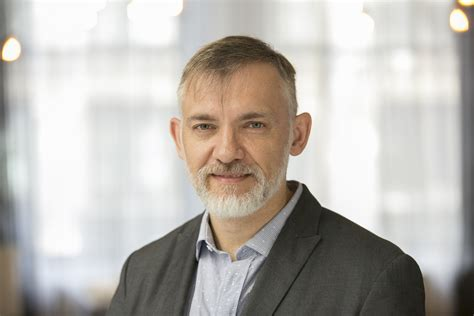
\includegraphics[scale=.13]{media/kapustin}
		\hspace*{1cm}
		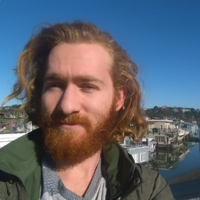
\includegraphics[scale=.21]{media/thorngren}
	\end{center}

	\pause
%	\vskip 20pt

	\begin{result}
		Effective construction of Adem coboundaries.
	\end{result}

	The above is joint with G. Brumfiel (Stanford) and J. Morgan (Columbia).

	\begin{center}
		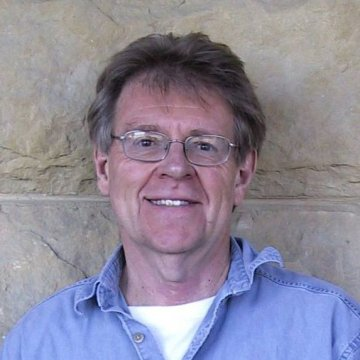
\includegraphics[scale=.21]{media/brumfiel}
		\hspace*{1cm}
		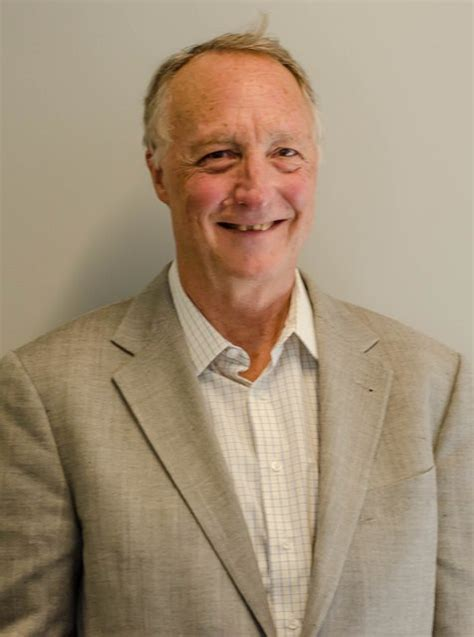
\includegraphics[scale=.09]{media/morgan}
	\end{center}
\end{frame}